\documentclass[aspectratio=169,xcolor=table]{beamer}
% Estilo compartilhado pelas aulas (incluído com \input{../estilo})
% Usa o template institucional (template/Estilo.sty: Madrid + orchid) e acrescenta
% apenas o necessário para figuras, pseudocódigo e código.
\usepackage{template/Estilo}
\graphicspath{{template/images/}}
\IfFileExists{portuguese.ldf}{\usepackage[brazilian]{babel}}{}
\usepackage{lmodern}
\usepackage{amsmath,amssymb,mathtools}
\usepackage{array}
\usepackage{tikz}
\usetikzlibrary{arrows.meta,positioning,calc,shapes.geometric,decorations.pathreplacing}
\usepackage[noend]{algpseudocode}

% ---------- Cores ----------
\definecolor{azul}{rgb}{0.2,0.2,0.7}
\colorlet{azulclaro}{azul!12}
\definecolor{laranja}{HTML}{D9622B}
\definecolor{verde}{HTML}{2E7D32}
\definecolor{vermelho}{HTML}{C62828}
\definecolor{cinza}{HTML}{6B6B6B}
\definecolor{roxo}{HTML}{6A1B9A}

% Tema em verde (tom da marca UDESC) no lugar do azul padrão do Madrid
\definecolor{verdetema}{HTML}{1E6B34}
\usecolortheme[named=verdetema]{structure}

% Blocos de exemplo/alerta (exemplo em azul para não se confundir com o tema)
\setbeamercolor{block title example}{fg=white,bg=azul}
\setbeamercolor{block body example}{bg=azul!8}
\setbeamercolor{block title alerted}{fg=white,bg=laranja}
\setbeamercolor{block body alerted}{bg=laranja!8}

% Agenda no início de cada seção, destacando a seção atual
\AtBeginSection[]{
  \begin{frame}
    \frametitle{Agenda da apresentação}
    \tableofcontents[currentsection]
  \end{frame}
}

% ---------- Código ----------
\lstset{
  language=Java,
  basicstyle=\ttfamily\footnotesize,
  keywordstyle=\color{azul}\bfseries,
  commentstyle=\color{cinza}\itshape,
  stringstyle=\color{verde},
  showstringspaces=false,
  columns=fullflexible,
  keepspaces=true,
  frame=single,
  rulecolor=\color{azulclaro},
  backgroundcolor=\color{azulclaro!30},
  literate={á}{{\'a}}1 {é}{{\'e}}1 {í}{{\'i}}1 {ó}{{\'o}}1 {ú}{{\'u}}1
           {ã}{{\~a}}1 {õ}{{\~o}}1 {ç}{{\c c}}1 {â}{{\^a}}1 {ê}{{\^e}}1 {ô}{{\^o}}1
}

% ---------- Pseudocódigo em português ----------
\algrenewcommand\algorithmicwhile{\textbf{enquanto}}
\algrenewcommand\algorithmicdo{\textbf{faça}}
\algrenewcommand\algorithmicfor{\textbf{para}}
\algrenewcommand\algorithmicforall{\textbf{para todo}}
\algrenewcommand\algorithmicif{\textbf{se}}
\algrenewcommand\algorithmicthen{\textbf{então}}
\algrenewcommand\algorithmicelse{\textbf{senão}}
\algrenewcommand\algorithmicreturn{\textbf{retorne}}
\algrenewcommand\algorithmicrepeat{\textbf{repita}}
\algrenewcommand\algorithmicuntil{\textbf{até que}}
\algrenewcommand\algorithmicprocedure{\textbf{procedimento}}
\algrenewcommand\algorithmicfunction{\textbf{função}}
\algrenewcommand\algorithmicend{\textbf{fim}}

% ---------- Estilos TikZ ----------
\tikzset{
  cli/.style={circle,draw=azul,fill=azulclaro,thick,inner sep=0pt,minimum size=5mm,font=\scriptsize},
  dep/.style={rectangle,draw=laranja,fill=laranja!25,thick,inner sep=0pt,minimum size=5.5mm,font=\scriptsize\bfseries},
  pt/.style={circle,fill=azul,inner sep=0pt,minimum size=2mm},
  aresta/.style={-{Stealth[length=2mm]},thick,azul},
  arestaB/.style={-{Stealth[length=2mm]},thick,laranja},
  arestaC/.style={-{Stealth[length=2mm]},thick,verde},
  removida/.style={thick,dashed,vermelho},
  nova/.style={very thick,verde},
}

% ---------- Atalhos ----------
\newcommand{\destaque}[1]{\textcolor{laranja}{\textbf{#1}}}
\newcommand{\nota}[1]{{\color{cinza}\footnotesize #1}}
\newcommand{\fonte}[1]{{\color{cinza}\scriptsize Fonte: #1}}

% ---------- Capa (padrão do template) ----------
\institute[UDESC/CCT]{Universidade do Estado de Santa Catarina -- UDESC/CCT\\
  Departamento de Ciência da Computação -- DCC\\
  Programa de Pós-Graduação em Computação Aplicada -- PPGCA}
\date[]{Joinville -- SC, 2026/2}
\setbeamercovered{dynamic}
% Logos com a mesma altura, centralizadas verticalmente e agrupadas no centro
\titlegraphic{
  \vspace*{-0.3cm}
  \adjustbox{valign=c}{
\includegraphics[height=0.65cm]{ppgca}}\hspace{1.2cm}%
  \adjustbox{valign=c}{
\includegraphics[height=0.85cm]{marcaudesc}}\hspace{1.2cm}%
  \adjustbox{valign=c}{
\includegraphics[height=0.65cm]{dcclogo}}
}


\title[Problema de Roteamento de Veículos]{Otimização Combinatória e o\\Problema de Roteamento de Veículos}
\subtitle{Aula 2 de 2}
\author[Kawan Weege]{\textbf{Kawan Weege}\\{\small Orientador: Prof. Dr. Fabiano Baldo}}

% Solução de exemplo usada em vários slides
\newcommand{\solucaoexemplo}{%
  \node[dep] (d) at (0,0) {D};
  \foreach \n/\x/\y in {a1/-1/1.5, a2/-2.2/2.4, a3/-3/1, a4/-2/0.2,
                        b1/1/2, b2/2.2/2.8, b3/3.2/1.5, b4/2.2/0.6,
                        c1/0.5/-1.5, c2/2/-2, c3/-0.5/-2.6, c4/-2/-1.6}
    \node[cli] (\n) at (\x,\y) {};
}

\begin{document}

% =====================================================================
\begin{frame}
  \titlepage
\end{frame}

\begin{frame}{Agenda da apresentação}
  \tableofcontents
\end{frame}

\begin{frame}{Revisão da aula anterior}
  \begin{itemize}
    \item \textbf{Otimização combinatória}: escolher a melhor entre um número finito, mas gigantesco, de soluções
    \item \textbf{TSP}: menor ciclo que visita todas as cidades
    \item \textbf{Construtivas}: vizinho mais próximo, inserção mais barata
    \item \textbf{Busca local}: 2-opt, relocate, swap $\Rightarrow$ ótimo local
    \item \textbf{Metaheurísticas}: ILS, SA, \dots\ para escapar de ótimos locais
  \end{itemize}
\end{frame}

% =====================================================================
\section{Do TSP ao VRP}

\begin{frame}{E se tivermos uma frota?}
  \begin{columns}[c]
    \begin{column}{0.5\textwidth}
      \begin{itemize}
        \item Um \textbf{depósito} central
        \item Vários \textbf{clientes}, cada um com uma \textbf{demanda}
        \item Uma \textbf{frota} de veículos com capacidade limitada
        \item Cada veículo sai do depósito, atende alguns clientes e volta
      \end{itemize}
      \vspace{0.5em}
      \begin{block}{Decisões}
        \begin{enumerate}
          \item \textbf{Agrupamento}: quais clientes cada veículo atende?
          \item \textbf{Sequenciamento}: em que ordem? \nota{(um TSP por veículo!)}
        \end{enumerate}
      \end{block}
    \end{column}
    \begin{column}{0.45\textwidth}
      \centering
      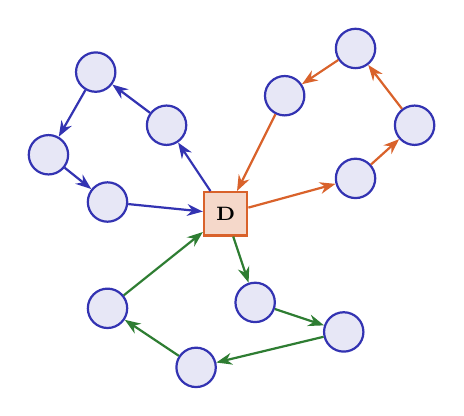
\begin{tikzpicture}[scale=0.75]
        \solucaoexemplo
        \draw[aresta] (d)--(a1); \draw[aresta] (a1)--(a2); \draw[aresta] (a2)--(a3); \draw[aresta] (a3)--(a4); \draw[aresta] (a4)--(d);
        \draw[arestaB] (d)--(b4); \draw[arestaB] (b4)--(b3); \draw[arestaB] (b3)--(b2); \draw[arestaB] (b2)--(b1); \draw[arestaB] (b1)--(d);
        \draw[arestaC] (d)--(c1); \draw[arestaC] (c1)--(c2); \draw[arestaC] (c2)--(c3); \draw[arestaC] (c3)--(c4); \draw[arestaC] (c4)--(d);
      \end{tikzpicture}\\\fonte{elaborado pelo autor.}
    \end{column}
  \end{columns}
\end{frame}

\begin{frame}{Por que o VRP importa?}
  \begin{itemize}
    \item \textbf{1959}: \citeonline{dantzig1959truck}, \emph{The Truck Dispatching Problem}: entrega de gasolina a postos
    \item Um dos problemas mais estudados da pesquisa operacional \cite{konstantakopoulos2022vrp,endler2023systematic}
    \item O transporte responde por 40--60\% dos custos logísticos \cite{aghaabdollahian2026overview}
  \end{itemize}
\end{frame}

\begin{frame}{Algumas aplicações}
  \begin{itemize}
    \item Distribuição de alimentos e bebidas \cite{ostermeier2021multi,polat2026enhanced}
    \item Coleta de lixo \cite{archetti2008split,ostermeier2021multi}
    \item Entregas de e-commerce (\emph{última milha}) \cite{aghaabdollahian2026overview}
    \item Transporte escolar \cite{gu2024multiple}
    \item Atendimento técnico e manutenção \cite{aghaabdollahian2026overview}
    \item Coleta de leite em fazendas \cite{alinaghian2018multi,gu2024multiple}
    \item Distribuição de combustível \cite{androutsopoulos2024fuel,baptista2024exact}
    \item Distribuição de ração animal \cite{archetti2008split,ostermeier2021multi}
  \end{itemize}
\end{frame}

% =====================================================================
\section{CVRP: restrição de capacidade}

\begin{frame}{Definição do CVRP \cite{dantzig1959truck,uchoa2017x}}
  \begin{columns}[T]
    \begin{column}{0.52\textwidth}
      \begin{block}{Dados}
        \begin{itemize}
          \item Grafo completo $G = (V, E)$, $V = \{0, 1, \dots, n\}$
          \item Vértice $0$: \textbf{depósito}
          \item Clientes $C = \{1, \dots, n\}$, cada um com \textbf{demanda} $q_i > 0$
          \item Custo (distância) $d_{ij}$ entre $i$ e $j$
          \item $K$ veículos idênticos com \textbf{capacidade} $Q$
        \end{itemize}
      \end{block}
    \end{column}
    \begin{column}{0.45\textwidth}
      \begin{block}{Uma solução é um conjunto de rotas tal que}
        \begin{itemize}
          \item cada rota começa e termina no depósito
          \item cada cliente é atendido por \textbf{exatamente uma} rota
          \item a demanda total de cada rota é $\le Q$
          \item são usadas no máximo $K$ rotas
        \end{itemize}
      \end{block}
    \end{column}
  \end{columns}
  \vspace{0.5em}
  \begin{center}
    \textbf{Objetivo}: minimizar a distância total percorrida.\\
    \nota{Variante comum: primeiro minimizar o número de veículos, depois a distância.}
  \end{center}
\end{frame}

\begin{frame}{Exemplo: capacidade $Q = 10$}
  \begin{columns}[c]
    \begin{column}{0.48\textwidth}
      \centering
      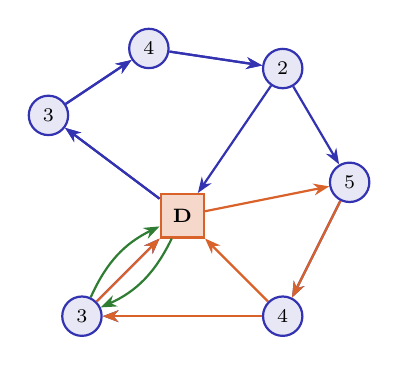
\begin{tikzpicture}[scale=0.85]
        \node[dep] (d) at (0,0) {D};
        \node[cli] (1) at (-2,1.5) {3};
        \node[cli] (2) at (-0.5,2.5) {4};
        \node[cli] (3) at (1.5,2.2) {2};
        \node[cli] (4) at (2.5,0.5) {5};
        \node[cli] (5) at (1.5,-1.5) {4};
        \node[cli] (6) at (-1.5,-1.5) {3};
        \draw<1>[aresta] (d)--(1); \draw<1>[aresta] (1)--(2); \draw<1>[aresta] (2)--(3);
        \draw<1>[aresta] (3)--(4); \draw<1>[aresta] (4)--(5); \draw<1>[aresta] (5)--(6); \draw<1>[aresta] (6)--(d);
        \draw<2->[aresta] (d)--(1); \draw<2->[aresta] (1)--(2); \draw<2->[aresta] (2)--(3); \draw<2->[aresta] (3)--(d);
        \draw<2->[arestaB] (d)--(4); \draw<2->[arestaB] (4)--(5);
        \draw<2>[arestaB] (5)--(6); \draw<2>[arestaB] (6)--(d);
        \draw<3->[arestaB] (5)--(d);
        \draw<3->[arestaC] (d) to[bend left=20] (6); \draw<3->[arestaC] (6) to[bend left=20] (d);
      \end{tikzpicture}\\\fonte{elaborado pelo autor.}\\
      \nota{O número dentro de cada cliente é sua demanda.}
    \end{column}
    \begin{column}{0.48\textwidth}
      \only<1>{
        \begin{alertblock}{Uma rota só (como no TSP)}
          Carga $= 3+4+2+5+4+3 = 21 > 10$\\
          \textbf{Inviável!}
        \end{alertblock}
        Precisamos de pelo menos $\lceil 21 / 10 \rceil = 3$ veículos?
      }
      \only<2>{
        \begin{alertblock}{Duas rotas}
          \textcolor{azul}{Rota 1}: $3+4+2 = 9 \le 10$ \checkmark\\
          \textcolor{laranja}{Rota 2}: $5+4+3 = 12 > 10$ \quad \textbf{inviável!}
        \end{alertblock}
        Limite inferior: $\lceil 21 / 10 \rceil = 3$ rotas.
      }
      \only<3>{
        \begin{block}{Três rotas}
          \textcolor{azul}{Rota 1}: $3+4+2 = 9 \le 10$ \checkmark\\
          \textcolor{laranja}{Rota 2}: $5+4 = 9 \le 10$ \checkmark\\
          \textcolor{verde}{Rota 3}: $3 \le 10$ \checkmark\\
          \textbf{Viável!}
        \end{block}
        Atinge o limite inferior de $\lceil 21 / 10 \rceil = 3$ rotas.
      }
    \end{column}
  \end{columns}
\end{frame}

\begin{frame}{Formulação matemática (dois índices)}
  $x_{ij} = 1$ se algum veículo vai diretamente de $i$ para $j$; $0$ caso contrário \cite{laporte1985optimal}.
  \begin{align*}
    \min\quad & \sum_{i \in V}\sum_{j \in V \setminus \{i\}} d_{ij}\, x_{ij} \\
    \text{s.a.}\quad
      & \textstyle\sum_{j \in V \setminus \{i\}} x_{ij} = 1 && \forall i \in C\\
      & \textstyle\sum_{j \in V \setminus \{i\}} x_{ji} = 1 && \forall i \in C\\
      & \textstyle\sum_{j \in C} x_{0j} \le K \\
      & \textstyle\sum_{i \in V \setminus S}\sum_{j \in S} x_{ij} \ge \left\lceil \frac{\sum_{h \in S} q_h}{Q} \right\rceil && \forall S \subseteq C,\ S \neq \emptyset\\
      & x_{ij} \in \{0,1\} && \forall i, j \in V,\ i \neq j
  \end{align*}
  \nota{A última restrição exige que pelo menos $\lceil \sum_{h \in S} q_h / Q \rceil$ veículos entrem em $S$: garante a capacidade e elimina subciclos.}
\end{frame}

% =====================================================================
\section{Uma segunda restrição: duração máxima}

\begin{frame}{Duração (ou distância) máxima da rota}
  \begin{columns}[c]
    \begin{column}{0.55\textwidth}
      \begin{block}{DCVRP --- \emph{Distance-Constrained CVRP}}
        Cada rota tem um limite $L$ de distância \cite{aghaabdollahian2026overview}; com tempos de serviço, vira um limite de duração:
        \[
          \sum_{(i,j) \in \text{rota}} d_{ij} \; + \sum_{i \in \text{rota}} s_i \;\le\; L
        \]
        \nota{$s_i$ = tempo de serviço no cliente $i$ (descarregar, por exemplo).}
      \end{block}
      \begin{itemize}
        \item Motivação: jornada de trabalho do motorista, autonomia de veículos elétricos ou drones, produtos perecíveis
        \item Hoje vamos usar $s_i = 0$: duração $=$ distância
      \end{itemize}
    \end{column}
    \begin{column}{0.42\textwidth}
      \centering
      \textbf{Exemplo}: $L = 25$, $s_i = 0$\\[0.5em]
      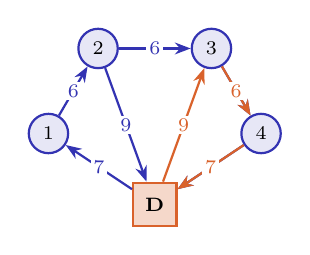
\begin{tikzpicture}[scale=0.9, dist/.style={font=\scriptsize, fill=white, inner sep=1pt}]
        \node[dep] (d) at (0,0) {D};
        \node[cli] (1) at (-1.5,1) {1};
        \node[cli] (2) at (-0.8,2.2) {2};
        \node[cli] (3) at (0.8,2.2) {3};
        \node[cli] (4) at (1.5,1) {4};
        \draw[aresta] (d)--(1) node[dist, midway] {7};
        \draw[aresta] (1)--(2) node[dist, midway] {6};
        \draw<1>[aresta] (2)--(3) node[dist, midway] {6};
        \draw<2->[aresta] (2)--(d) node[dist, midway] {9};
        \draw<1>[aresta] (3)--(4) node[dist, midway] {6};
        \draw<1>[aresta] (4)--(d) node[dist, midway] {7};
        \draw<2->[arestaB] (d)--(3) node[dist, midway] {9};
        \draw<2->[arestaB] (3)--(4) node[dist, midway] {6};
        \draw<2->[arestaB] (4)--(d) node[dist, midway] {7};
      \end{tikzpicture}\\\fonte{elaborado pelo autor.}\\[0.5em]
      \only<1>{
        Uma rota: $7+6+6+6+7 = 32 > 25$\\
        \textbf{Inviável!}
      }
      \only<2>{
        \textcolor{azul}{Rota 1}: $7+6+9 = 22 \le 25$ \checkmark\\
        \textcolor{laranja}{Rota 2}: $9+6+7 = 22 \le 25$ \checkmark
      }
    \end{column}
  \end{columns}
\end{frame}

\begin{frame}{A família VRP}
  \small
  \begin{columns}[T]
    \begin{column}{0.48\textwidth}
      \begin{itemize}
        \item \textbf{VRPTW}: janelas de tempo $[a_i, b_i]$ para atender cada cliente \cite{solomon1987algorithms}
        \item \textbf{MDVRP}: vários depósitos \cite{tillman1969multiple}
        \item \textbf{HFVRP}: frota heterogênea (capacidades e custos diferentes) \cite{golden1984fleet}
        \item \textbf{PDP}: coleta e entrega (ex.: Uber, transporte de pacientes) \cite{savelsbergh1995general}
      \end{itemize}
    \end{column}
    \begin{column}{0.48\textwidth}
      \begin{itemize}
        \item \textbf{SDVRP}: entrega fracionada (um cliente pode ser atendido por mais de um veículo) \cite{dror1989savings}
        \item \textbf{MCVRP}: veículos com vários compartimentos \cite{brown1981realtime}
        \item \textbf{MTVRP}: múltiplas viagens por veículo \cite{fleischmann1990vehicle}
        \item \textbf{VRP dinâmico / estocástico}: pedidos ou tempos de viagem incertos \cite{psaraftis1988dynamic,tillman1969multiple}
      \end{itemize}
    \end{column}
  \end{columns}
  \vspace{1em}
  \begin{block}{\emph{VRPs Ricos}}
    Essas são apenas algumas: a literatura classifica mais de 30 variantes do VRP \cite{aghaabdollahian2026overview}.
    Problemas reais combinam várias dessas características ao mesmo tempo.
  \end{block}
\end{frame}

% =====================================================================
\section{Representação e viabilidade}

\begin{frame}{Como representar uma solução?}
  \begin{columns}[c]
    \begin{column}{0.45\textwidth}
      \begin{block}{Lista de rotas}
        \centering
        \ttfamily
        R1: [3, 7, 1]\\
        R2: [5, 2]\\
        R3: [4, 6, 8]
      \end{block}
    \end{column}
    \begin{column}{0.5\textwidth}
      \begin{itemize}
        \item Cada rota é uma sequência de clientes
        \item O depósito no início e no fim é implícito
      \end{itemize}
    \end{column}
  \end{columns}
  \vspace{1em}
  \begin{block}{Outras representações}
    \small
    \begin{itemize}
      \item Rota gigante com delimitadores: \texttt{[3, 7, 1, 0, 5, 2, 0, 4, 6, 8]} \cite{alinaghian2018multi}
      \item Rota gigante sem delimitadores + \emph{Split}: \texttt{[3, 7, 1, 5, 2, 4, 6, 8]} \cite{beasley1983route,prins2004split}
    \end{itemize}
  \end{block}
\end{frame}

\begin{frame}{Soluções inviáveis: rejeitar ou penalizar?}
  \begin{columns}[T]
    \begin{column}{0.48\textwidth}
      \begin{block}{Rejeitar}
        Só aceita movimentos que mantêm a solução viável.
        \begin{itemize}
          \item Simples
          \item Mas o espaço viável pode ser ``fragmentado'': a busca fica presa
        \end{itemize}
      \end{block}
      \vspace{1em}
      \centering
      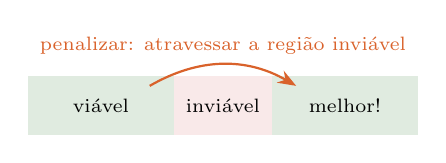
\begin{tikzpicture}[scale=0.62]
        \fill[verde!15] (0,0) rectangle (3,1.2); \node[font=\scriptsize] at (1.5,0.6) {viável};
        \fill[vermelho!10] (3,0) rectangle (5,1.2); \node[font=\scriptsize] at (4,0.6) {inviável};
        \fill[verde!15] (5,0) rectangle (8,1.2); \node[font=\scriptsize] at (6.5,0.6) {melhor!};
        \draw[-{Stealth},thick,laranja] (2.5,1.0) to[bend left=30] node[above,font=\scriptsize] {penalizar: atravessar a região inviável} (5.5,1.0);
      \end{tikzpicture}\\\fonte{elaborado pelo autor.}
    \end{column}
    \begin{column}{0.48\textwidth}
      \begin{block}{Penalizar}
        Aceita soluções inviáveis, mas paga por isso:
        \[
          f(s) = \text{dist}(s) + \alpha\, E_Q(s) + \beta\, E_L(s)
        \]
        \nota{$E_Q$, $E_L$: quanto a solução excede a capacidade e a duração máxima.}
        \begin{itemize}
          \item $\alpha, \beta$ ajustados dinamicamente
          \item Usado pelos melhores métodos \cite{cordeau1997tabu,vidal2022hgs}
        \end{itemize}
      \end{block}
    \end{column}
  \end{columns}
\end{frame}

% =====================================================================
\section{Heurísticas construtivas}

\begin{frame}{Vizinho mais próximo (versão VRP)}
  \begin{columns}[c]
    \begin{column}{0.58\textwidth}
      \begin{algorithmic}[1]
        \State $rotas \gets \emptyset$
        \While{há clientes não atendidos}
          \State $r \gets$ rota vazia; $atual \gets 0$
          \Loop
            \State $c \gets$ cliente não atendido mais próximo de $atual$ \textbf{que cabe} em $r$
            \If{não existe $c$} \textbf{break} \EndIf
            \State adicione $c$ ao fim de $r$; $atual \gets c$
          \EndLoop
          \State adicione $r$ a $rotas$
        \EndWhile
      \end{algorithmic}
    \end{column}
    \begin{column}{0.4\textwidth}
      \begin{block}{``Cabe'' significa}
        \small
        \begin{itemize}
          \item $\text{carga}(r) + q_c \le Q$
          \item $\text{dist}(r) - d_{atual,0}$\\ $\quad + d_{atual,c} + d_{c,0} \le L$
        \end{itemize}
      \end{block}
    \end{column}
  \end{columns}
\end{frame}

\begin{frame}{Vizinho mais próximo: exemplo com $Q = 10$}
  \begin{columns}[c]
    \begin{column}{0.55\textwidth}
      \centering
      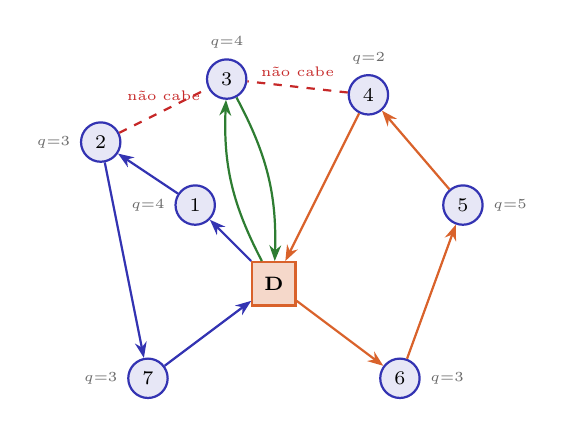
\begin{tikzpicture}[scale=1.0, dem/.style={font=\tiny, text=cinza}]
        \node[dep] (d) at (0,0) {D};
        \node[cli, label={[dem]left:$q{=}4$}]  (1) at (-1.0,1.0) {1};
        \node[cli, label={[dem]left:$q{=}3$}]  (2) at (-2.2,1.8) {2};
        \node[cli, label={[dem]above:$q{=}4$}] (3) at (-0.6,2.6) {3};
        \node[cli, label={[dem]above:$q{=}2$}] (4) at (1.2,2.4) {4};
        \node[cli, label={[dem]right:$q{=}5$}] (5) at (2.4,1.0) {5};
        \node[cli, label={[dem]right:$q{=}3$}] (6) at (1.6,-1.2) {6};
        \node[cli, label={[dem]left:$q{=}3$}]  (7) at (-1.6,-1.2) {7};
        % rota 1
        \draw<2->[aresta] (d)--(1);
        \draw<3->[aresta] (1)--(2);
        \draw<4>[removida] (2)--(3) node[midway, above, font=\tiny, vermelho] {não cabe};
        \draw<4->[aresta] (2)--(7);
        \draw<5->[aresta] (7)--(d);
        % rota 2
        \draw<6->[arestaB] (d)--(6);
        \draw<6->[arestaB] (6)--(5);
        \draw<6->[arestaB] (5)--(4);
        \draw<6>[removida] (4)--(3) node[midway, above, font=\tiny, vermelho] {não cabe};
        \draw<6->[arestaB] (4)--(d);
        % rota 3
        \draw<7->[arestaC] (d) to[bend left=15] (3);
        \draw<7->[arestaC] (3) to[bend left=15] (d);
      \end{tikzpicture}\\\fonte{elaborado pelo autor.}
    \end{column}
    \begin{column}{0.42\textwidth}
      \small
      \only<1>{
        Começamos uma rota vazia no depósito.\\[0.5em]
        \textcolor{azul}{Rota 1}: carga $0$
      }
      \only<2>{
        Mais próximo de D: cliente 1.\\
        $0 + 4 = 4 \le 10$ \checkmark\\[0.5em]
        \textcolor{azul}{Rota 1}: [1], carga $4$
      }
      \only<3>{
        Mais próximo de 1: cliente 2.\\
        $4 + 3 = 7 \le 10$ \checkmark\\[0.5em]
        \textcolor{azul}{Rota 1}: [1, 2], carga $7$
      }
      \only<4>{
        Mais próximo de 2: cliente 3, mas\\
        $7 + 4 = 11 > 10$ \quad \textcolor{vermelho}{não cabe}\\[0.3em]
        Mais próximo \textbf{que cabe}: cliente 7.\\
        $7 + 3 = 10 \le 10$ \checkmark\\[0.5em]
        \textcolor{azul}{Rota 1}: [1, 2, 7], carga $10$
      }
      \only<5>{
        Nenhum cliente cabe: a rota volta ao depósito.\\[0.5em]
        \textcolor{azul}{Rota 1}: [1, 2, 7], carga $10$
      }
      \only<6>{
        Nova rota a partir do depósito: 6, 5 e 4.\\
        O cliente 3 não cabe: $10 + 4 > 10$.\\[0.5em]
        \textcolor{azul}{Rota 1}: [1, 2, 7], carga $10$\\
        \textcolor{laranja}{Rota 2}: [6, 5, 4], carga $10$
      }
      \only<7>{
        Só sobrou o cliente 3: ele fica sozinho em uma rota.\\[0.5em]
        \textcolor{azul}{Rota 1}: [1, 2, 7], carga $10$\\
        \textcolor{laranja}{Rota 2}: [6, 5, 4], carga $10$\\
        \textcolor{verde}{Rota 3}: [3], carga $4$
      }
    \end{column}
  \end{columns}
\end{frame}

\begin{frame}{Algoritmo de economias (Clarke \& Wright)}
  Une rotas enquanto isso reduzir a distância total \cite{clarke1964savings}.
  \begin{columns}[c]
    \begin{column}{0.55\textwidth}
      \centering
      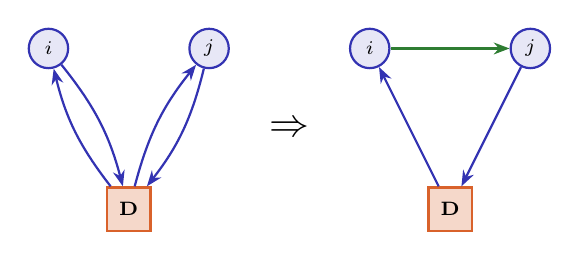
\begin{tikzpicture}[scale=0.85]
        \node[dep] (d) at (0,0) {D};
        \node[cli] (i) at (-1.2,2.4) {$i$};
        \node[cli] (j) at (1.2,2.4) {$j$};
        \draw[aresta,bend left=12] (d) to (i); \draw[aresta,bend left=12] (i) to (d);
        \draw[aresta,bend left=12] (d) to (j); \draw[aresta,bend left=12] (j) to (d);
        \node[font=\Large] at (2.4,1.2) {$\Rightarrow$};
        \begin{scope}[xshift=4.8cm]
          \node[dep] (d2) at (0,0) {D};
          \node[cli] (i2) at (-1.2,2.4) {$i$};
          \node[cli] (j2) at (1.2,2.4) {$j$};
          \draw[aresta] (d2)--(i2); \draw[nova,-{Stealth[length=2mm]}] (i2)--(j2); \draw[aresta] (j2)--(d2);
        \end{scope}
      \end{tikzpicture}\\\fonte{elaborado pelo autor.}
      \[
        s_{ij} = d_{0i} + d_{0j} - d_{ij}
      \]
      \nota{Quanto economizamos ao atender $j$ logo depois de $i$, em vez de voltar ao depósito.}
    \end{column}
    \begin{column}{0.43\textwidth}
      \small
      \begin{algorithmic}[1]
        \State crie uma rota $0 \to i \to 0$ para cada cliente
        \State calcule $s_{ij}$ para todo par $i<j$
        \State ordene os pares por $s_{ij}$ decrescente
        \ForAll{par $(i,j)$}
          \If{$i$ e $j$ estão em rotas diferentes, \textbf{nas extremidades}, e a rota unida é \textbf{viável}}
            \State una as duas rotas por $(i,j)$
          \EndIf
        \EndFor
      \end{algorithmic}
    \end{column}
  \end{columns}
\end{frame}

\begin{frame}{Clarke \& Wright: unindo rotas pelas extremidades}
  \begin{columns}[c]
    \begin{column}{0.5\textwidth}
      Se $i$ está no \textbf{fim} da rota $A$ e $j$ no \textbf{início} da rota $B$:
      \begin{center}
        \ttfamily\small
        A = [5, 3, \textcolor{laranja}{i}] \quad B = [\textcolor{laranja}{j}, 8, 2]\\[0.3em]
        $\Rightarrow$ [5, 3, \textcolor{laranja}{i}, \textcolor{laranja}{j}, 8, 2]
      \end{center}
      \vspace{0.5em}
      Nos outros casos, inverta uma das rotas antes (simétrico: o custo não muda).
      \vspace{0.5em}
      \begin{block}{Por que só extremidades?}
        \small
        Se $i$ estiver no meio da rota, ele já tem dois vizinhos: não há como ligá-lo a $j$ sem quebrar a rota.
      \end{block}
    \end{column}
    \begin{column}{0.45\textwidth}
      \begin{block}{Viabilidade da união}
        \begin{itemize}
          \item Carga: $\text{carga}(A) + \text{carga}(B) \le Q$
          \item Distância: \\
            \small$\text{dist}(A) + \text{dist}(B) - s_{ij} \le L$
        \end{itemize}
      \end{block}
      \nota{Repare: a economia $s_{ij}$ é exatamente a redução de distância ao unir as rotas.}
    \end{column}
  \end{columns}
\end{frame}

\begin{frame}{Outras construtivas}
  \begin{columns}[c]
    \begin{column}{0.55\textwidth}
      \begin{block}{Varredura (\emph{Sweep})}
        \small
        \citeonline{gillett1974sweep}:
        \begin{enumerate}
          \item Ordene os clientes pelo \textbf{ângulo polar} em relação ao depósito
          \item Gire uma ``semirreta'' adicionando clientes à rota atual até não caber mais
          \item Resolva um TSP em cada rota (ex.: 2-opt)
        \end{enumerate}
        \nota{\emph{Agrupar primeiro, rotear depois} (cluster-first, route-second).}
      \end{block}
      \begin{block}{Rotear primeiro, agrupar depois}
        \small
        Resolva um TSP com todos os clientes e corte a rota gigante com o \emph{Split} \cite{beasley1983route}.
      \end{block}
    \end{column}
    \begin{column}{0.4\textwidth}
      \centering
      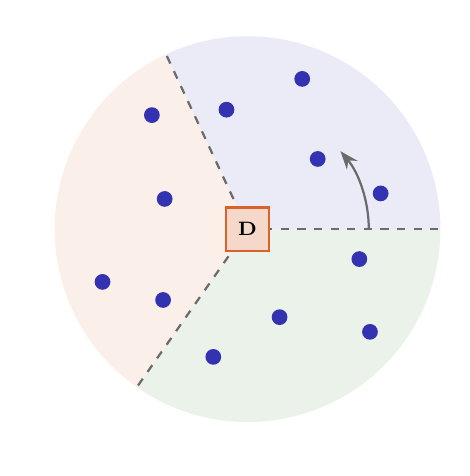
\begin{tikzpicture}[scale=0.7]
        \fill[azul!10] (0,0) -- (3.5,0) arc (0:115:3.5) -- cycle;
        \fill[laranja!10] (0,0) -- (115:3.5) arc (115:235:3.5) -- cycle;
        \fill[verde!10] (0,0) -- (235:3.5) arc (235:360:3.5) -- cycle;
        \draw[thick,cinza,dashed] (0,0) -- (3.5,0);
        \draw[thick,cinza,dashed] (0,0) -- (115:3.5);
        \draw[thick,cinza,dashed] (0,0) -- (235:3.5);
        \draw[-{Stealth},thick,cinza] (2.2,0) arc (0:40:2.2);
        \node[dep] at (0,0) {D};
        \foreach \a/\r in {15/2.5, 45/1.8, 70/2.9, 100/2.2, 130/2.7, 160/1.6, 200/2.8, 220/2.0, 255/2.4, 290/1.7, 320/2.9, 345/2.1}
          \node[pt] at (\a:\r) {};
      \end{tikzpicture}\\\fonte{elaborado pelo autor.}
    \end{column}
  \end{columns}
\end{frame}

% =====================================================================
\section{Busca local para o VRP}

\begin{frame}{Vizinhanças intra-rota e inter-rotas}
  \begin{columns}[T]
    \begin{column}{0.4\textwidth}
      \begin{block}{Intra-rota}
        Cada rota é um TSP: reutilize o que já sabemos!
        \begin{itemize}
          \item 2-opt \cite{croes1958method}
          \item relocate, swap, or-opt \cite{or1976traveling}
        \end{itemize}
        \nota{Só a duração pode mudar; a carga não.}
      \end{block}
    \end{column}
    \begin{column}{0.56\textwidth}
      \begin{block}{Inter-rotas}
        Movem clientes \textbf{entre} rotas: mudam o agrupamento.
        \begin{itemize}
          \item \textbf{Relocate}: move um cliente para outra rota \cite{osman1993metastrategy}
          \item \textbf{Swap}: troca dois clientes de rotas diferentes \cite{osman1993metastrategy}
          \item \textbf{2-opt*}: troca os ``finais'' de duas rotas \cite{potvin1995exchange}
          \item \textbf{Cross-exchange}: troca segmentos de duas rotas \cite{taillard1997tabu}
        \end{itemize}
        \nota{Carga \textbf{e} duração precisam ser verificadas.}
      \end{block}
    \end{column}
  \end{columns}
\end{frame}

\begin{frame}{Relocate inter-rotas}
  \begin{columns}[c]
    \begin{column}{0.55\textwidth}
      \centering
      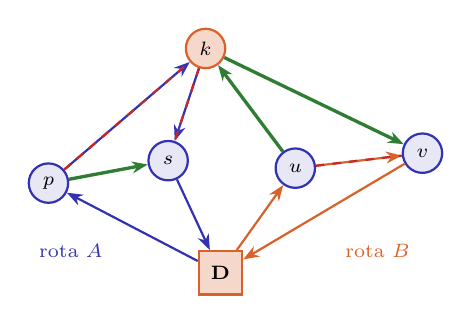
\begin{tikzpicture}[scale=0.95]
        \node[dep] (d) at (0,0) {D};
        \node[cli] (p) at (-2.3,1.2) {$p$};
        \node[cli,fill=laranja!25,draw=laranja] (k) at (-0.2,3.0) {$k$};
        \node[cli] (s) at (-0.7,1.5) {$s$};
        \node[cli] (u) at (1.0,1.4) {$u$};
        \node[cli] (v) at (2.7,1.6) {$v$};
        \draw[aresta] (d)--(p);
        \draw<1>[aresta] (p)--(k); \draw<1>[aresta] (k)--(s);
        \draw<2->[removida] (p)--(k); \draw<2->[removida] (k)--(s);
        \draw<2->[nova,-{Stealth[length=2mm]}] (p)--(s);
        \draw[aresta] (s)--(d);
        \draw[arestaB] (d)--(u);
        \draw<1>[arestaB] (u)--(v);
        \draw<2->[removida] (u)--(v);
        \draw<2->[nova,-{Stealth[length=2mm]}] (u)--(k);
        \draw<2->[nova,-{Stealth[length=2mm]}] (k)--(v);
        \draw[arestaB] (v)--(d);
        \node[azul,font=\scriptsize] at (-2.0,0.3) {rota $A$};
        \node[laranja,font=\scriptsize] at (2.1,0.3) {rota $B$};
      \end{tikzpicture}\\\fonte{elaborado pelo autor.}
    \end{column}
    \begin{column}{0.43\textwidth}
      \small
      Retira $k$ da rota $A$ (entre $p$ e $s$) e insere na rota $B$ entre $u$ e $v$.\\[0.5em]
      \textbf{Variação de distância}:
      \begin{align*}
        \Delta_A &= d_{ps} - d_{pk} - d_{ks}\\
        \Delta_B &= d_{uk} + d_{kv} - d_{uv}\\
        \Delta &= \Delta_A + \Delta_B
      \end{align*}
      \textbf{Viável se}:
      \begin{itemize}
        \item $\text{carga}(B) + q_k \le Q$
        \item $\text{dist}(B) + \Delta_B \le L$
      \end{itemize}
      \nota{A rota $A$ só fica mais curta e mais leve: continua viável (se a desigualdade triangular vale).}
    \end{column}
  \end{columns}
\end{frame}

\begin{frame}{Swap e 2-opt* inter-rotas}
  \begin{columns}[T]
    \begin{column}{0.48\textwidth}
      \centering
      \textbf{Swap}\\[0.3em]
      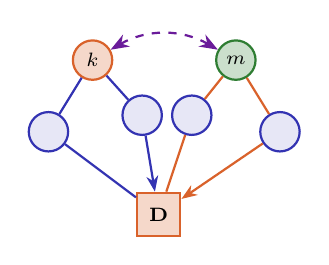
\begin{tikzpicture}[scale=0.7]
        \node[dep] (d) at (0,0) {D};
        \node[cli] (a1) at (-2,1.5) {};
        \node[cli,fill=laranja!25,draw=laranja] (a2) at (-1.2,2.8) {$k$};
        \node[cli] (a3) at (-0.3,1.8) {};
        \node[cli] (b1) at (0.6,1.8) {};
        \node[cli,fill=verde!25,draw=verde] (b2) at (1.4,2.8) {$m$};
        \node[cli] (b3) at (2.2,1.5) {};
        \draw[aresta] (d)--(a1)--(a2)--(a3)--(d);
        \draw[arestaB] (d)--(b1)--(b2)--(b3)--(d);
        \draw[{Stealth}-{Stealth},thick,dashed,roxo] (a2) to[bend left=30] (b2);
      \end{tikzpicture}\\
      \small Troca $k$ (rota $A$) com $m$ (rota $B$).\\
      Carga: $\text{carga}(A) - q_k + q_m \le Q$ e o análogo para $B$.
    \end{column}
    \begin{column}{0.48\textwidth}
      \centering
      \textbf{2-opt*}\\[0.3em]
      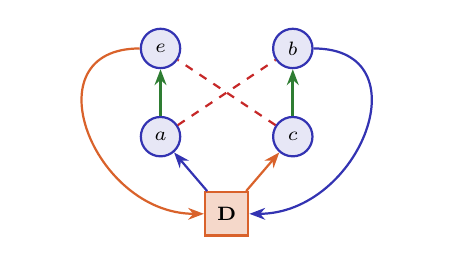
\begin{tikzpicture}[scale=0.7]
        \node[dep] (d) at (0,0) {D};
        \node[cli] (a) at (-1.2,1.4) {$a$};
        \node[cli] (e) at (-1.2,3.0) {$e$};
        \node[cli] (c) at (1.2,1.4) {$c$};
        \node[cli] (b) at (1.2,3.0) {$b$};
        \draw[aresta] (d)--(a);
        \draw[arestaB] (d)--(c);
        \draw[removida] (a)--(b); \draw[removida] (c)--(e);
        \draw[nova,-{Stealth[length=2mm]}] (a)--(e);
        \draw[nova,-{Stealth[length=2mm]}] (c)--(b);
        \draw[aresta] (b) to[out=0,in=0,looseness=1.6] (d);
        \draw[arestaB] (e) to[out=180,in=180,looseness=1.6] (d);
      \end{tikzpicture}\\
      \small Remove $(a,b)$ e $(c,e)$; liga $a \to e$ e $c \to b$:\\
      o início de cada rota passa a continuar com o final da outra.
    \end{column}
  \end{columns}
  {\centering\fonte{elaborado pelo autor.}\par}
\end{frame}

\begin{frame}{Juntando tudo: descida em vizinhanças variáveis (VND)}
  Explora as vizinhanças em ordem, voltando à primeira a cada melhora \cite{mladenovic1997variable}.
  \vspace{0.5em}
  \begin{algorithmic}[1]
    \State $N_1, \dots, N_m \gets$ lista de vizinhanças
    \State $k \gets 1$
    \While{$k \le m$}
      \State procure um vizinho $s' \in N_k(s)$ melhor que $s$
      \If{encontrou}
        \State $s \gets s'$; \ $k \gets 1$
      \Else
        \State $k \gets k + 1$
      \EndIf
    \EndWhile
    \State \Return $s$ \Comment{ótimo local para todas}
  \end{algorithmic}
\end{frame}

% =====================================================================
\section{Metaheurísticas}

\begin{frame}{Metaheurísticas mais usadas no VRP}
  As mais frequentes na literatura recente \cite{elshaer2020taxonomic,endler2023systematic}:
  \small
  \begin{block}{Baseadas em uma solução}
    \begin{itemize}
      \item \textbf{Busca Tabu}: aceita pioras e proíbe movimentos recentes \cite{glover1986future}
      \item \textbf{VNS}: perturbação + busca local em várias vizinhanças \cite{mladenovic1997variable}
      \item \textbf{ILS}: perturbação + busca local \cite{lourenco2003iterated}
      \item \textbf{Simulated Annealing}: aceita pioras com probabilidade decrescente \cite{kirkpatrick1983optimization}
      \item \textbf{ALNS}: destrói parte da solução e a reconstrói \cite{ropke2006alns}
    \end{itemize}
  \end{block}
  \begin{block}{Baseadas em população}
    \begin{itemize}
      \item \textbf{Algoritmo genético}: cruzamento e mutação de soluções \cite{holland1975adaptation}
      \item \textbf{Colônia de formigas}: rotas construídas a partir de feromônios \cite{dorigo1996ant}
    \end{itemize}
  \end{block}
\end{frame}

% =====================================================================
\section{Exercício prático}

\begin{frame}{Exercício}
  Código inicial em Java: \texttt{aula-2/exercicio/}. Compile com \texttt{javac *.java} e rode \texttt{java Main}.
  \vspace{0.5em}
  \begin{enumerate}
    \item Implemente \texttt{Rota.carga()}, \texttt{Rota.distancia()} (\alert{saindo e voltando ao depósito})\\
      e \texttt{Rota.ehViavel()} (capacidade $Q$ \textbf{e} distância máxima $L$).\\
      \nota{Teste: \texttt{Solucao.validar()} (já pronta) confere a solução.}
    \item Implemente \texttt{VizinhoMaisProximo.construir()} respeitando as duas restrições.
    \item Implemente \texttt{RelocateInter.melhorar()} com primeira melhora.\\
      \nota{O 2-opt intra-rota já está pronto.}
    \item Rode o \texttt{Main} e preencha a tabela:
  \end{enumerate}
  \begin{center}
  \small
  \begin{tabular}{lccc}
    \toprule
    & VMP & VMP + 2-opt & VMP + 2-opt + Relocate \\
    \midrule
    50 clientes & distância / rotas & distância / rotas & distância / rotas \\
    \bottomrule
  \end{tabular}
  \end{center}
  \nota{O programa gera arquivos \texttt{.svg} com as rotas.}
\end{frame}

\begin{frame}{Para continuar estudando}
  \begin{block}{Leituras}
    \begin{itemize}
      \item \citeonline{toth2014vrp}: \emph{Vehicle Routing: Problems, Methods, and Applications}
      \item \citeonline{elshaer2020taxonomic}: taxonomia de metaheurísticas para o VRP
      \item \citeonline{konstantakopoulos2022vrp}: classificação de variantes e algoritmos em 263 artigos
      \item \citeonline{endler2023systematic}: revisão sistemática das publicações recentes
      \item \citeonline{aghaabdollahian2026overview}: revisão com mais de 30 variantes do VRP
      \item Variantes específicas: \citeonline{archetti2008split} (SDVRP), \citeonline{ostermeier2021multi} (MCVRP), \citeonline{gu2024multiple} (múltiplas commodities)
    \end{itemize}
  \end{block}
  \vspace{0.5em}
  \begin{block}{Ferramentas e instâncias}
    \begin{itemize}
      \item PyVRP (\texttt{pyvrp.org}): biblioteca de código aberto com HGS
      \item CVRPLIB: \texttt{vrp.galgos.inf.puc-rio.br}
    \end{itemize}
  \end{block}
\end{frame}

\section*{Referências}
\begin{frame}[allowframebreaks]
  \frametitle{Referências Bibliográficas}
  {\footnotesize
    \bibliography{referencias}
  }
\end{frame}

% Repetir o slide de título no final
\begin{frame}
  \titlepage
\end{frame}

\end{document}
